\chapter{Introdução}
\label{chap:intro}

Os robôs móveis têm a capacidade de se moverem sob seu próprio controle. Quando o robô é capaz de executar tarefas usando estado físico e/ou sensores sem intervenção humana é categorizado como autônomo, conforme às definições da norma \cite{ISO}. De acordo com \cite{Rubio} plataformas móveis podem ser classificados,quanto ao sistema de locomoção, como terrestres, aquáticos e aéreos. Os terrestres são subdivididos em robôs que possuem rodas, pernas (bípedes) ou esteiras. Cada um desses métodos possuem características especifícas quanto ao movimento a ser realizado. Os bípedes, por exemplo, simulam um caminhar antropomórfico, semelhante aos humanos. 

O desenvolvimento deste projeto consiste em produzir um robô que possa caminhar sobre duas pernas. Além disso, o walker deve se locomover de forma autonôma a fim de realizar uma dada missão.
Neste capítulo serão abordados os requisitos do cliente, os requisistos técnicos, a missão do robô e a pesquisa por similares. 


\section{Objetivo}
\label{sec:obj}

O estudo bibliográfico foi realizado com o intuito de auxiliar no desenvolvimento do projeto Walker que tem como objetivo construir um robô humanóide de pequeno porte. Esta pesquisa visa contribuir com informações obtidas através das análise das principais características dos sistemas dos robôs humanoídes já existentes. 

Durante a ideação do projeto fez-se necessário realizar uma pesquisa por tecnologias similares, a fim de estudar seu funcionamento e características. Dessa forma, foram reunidos robôs de pequeno porte que se locomovessem sobre pernas, de maneira autonôma.

Desta maneira, os modelos relevantes a este projeto foram detalhados a seguir. 

\section{Justificativa}
\label{sec:justi}

Robôs antropomórficos são amplamente utilizados em diversas áreas no dia-a-dia, desde interações com humanos até aplicações na área da saúde, bem como em pesquisas acadêmicas, sendo uma configuração mais adequada para transposição de ambientes de difícil navegação.
Além disso, faz-se necessário o fomento ao desenvolvimento da Robótica no estado da Bahia, bem como o estudo de robôs antropomórficos dentro da Instituição Senai Cimatec, elevando seu nível competitivo.

Desta forma, é idealizado um robô bípede de pequeno porte, capaz de navegar e explorar em uma área delimitada de forma autônoma.


%*******************************************************************

% \chapter{Ambiente de desenvolvimento}
% \label{chap:fund}


% \section{Ambiente de aplicação}
% \label{sec:fun1}

% \section{Situação atual no desenvolvimento de Robôs Bípedes}
% \label{sec:fun2}

% \section{Mercado de atuação}
% \label{sec:fun3}

%*******************************************************************

\chapter{Metodologia}
\label{chap:metod}

\section{Método bili}
\label{sec:bili}

O método BILI (Bibliographic and Literary Review Method) é uma metodologia de pesquisa para o estudo das revisões bibliográficas que visa otimizar a busca e a seleção das referências. Este método é composto por quatro fases e utiliza  ferramentas como o  Rstudio, o Cmaptools e o Mendeley para a seleção, revisão e organização das documentações encontradas. Através desta metodologia é possível encontrar os artigos e autores mais relevantes para a pesquisa.

\begin{figure} [H]	
    \centering
    \caption{Fases do método BILI}
    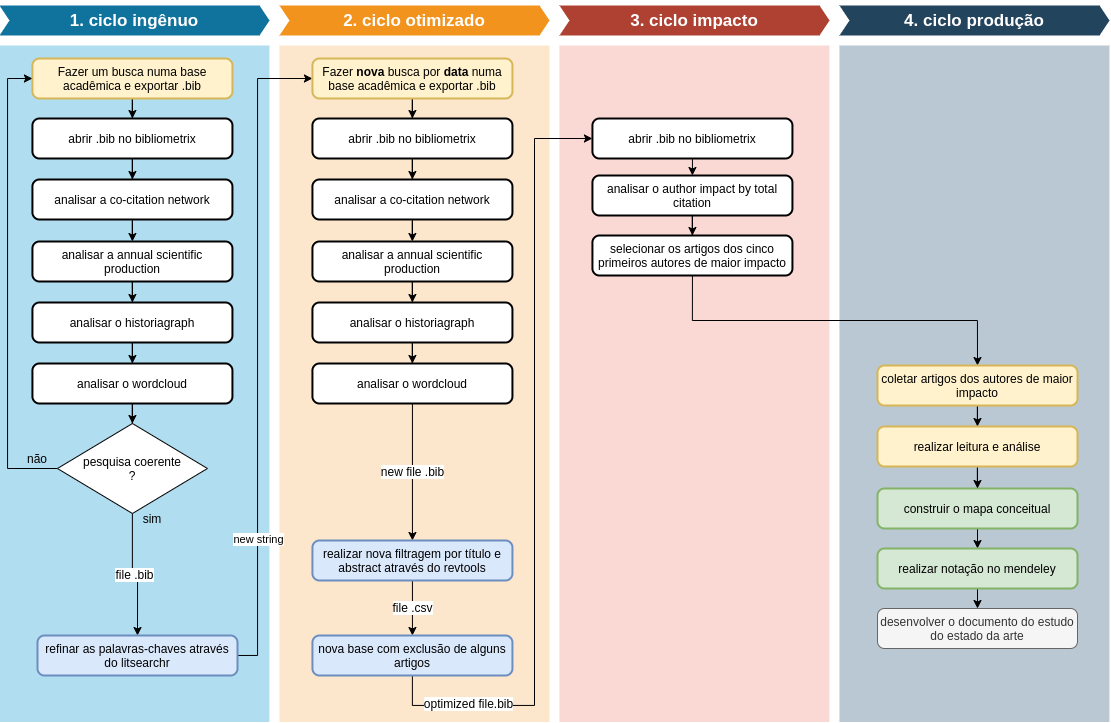
\includegraphics[width=0.6\textwidth]{bili}
    % \caption*{Fonte: Autoria própria.}
    \label{fig:bili}
\end{figure}

\subsection{Fase 1}
\label{sec:fase1}

A primeira fase é denominada de ciclo ingênuo e corresponde a pesquisa inicial feita em uma base acadêmica  de onde é exportado o arquivo .bib. Através deste arquivo utilizando a ferramenta biblioshiny, fornecida pelo pacote Bibliometrix, é feita uma análise da rede de co-citação, da produção cientifica anual e das palavras que aparecem com maior frequência nos artigos. Caso estas informações estejam coerentes com a pesquisa desejada, o pacote litsearchr é utilizado para auxiliar no refinamento da pesquisa através das palavras-chaves. Se o resultado obtido não for satisfatório a busca na base acadêmica deve ser refeita. E, por fim, é gerada uma nova string que será utilizada para realizar uma nova busca. 


\subsection{Fase 2}
\label{sec:fase2}

A fase dois é chamada de ciclo otimizado pois, nesta fase é feita uma nova busca na base acadêmica porém, utilizando as palavras-chaves refinadas. Desta forma, o passo seguinte é realizar a mesma análise feita no primeiro ciclo e, após está análise é feita uma filtragem dos artigos utilizando o Revtools. Esta ferramenta permite o pesquisador selecionar os melhores artigos para sua pesquisa através da leitura dos títulos e abstracts. E, então é exportado um novo arquivo .bib com os dados otimizados para a pesquisa. 

\subsection{Fase 3}
\label{sec:fase3}

Na terceira fase, denominada ciclo impacto, é feita a análise do imapcto do autor utilizando o bibliometrix. E, então são selecionados os artigos dos cinco primeiros autores de maior impacto.

\subsection{Fase 4}
\label{sec:fase4}

Na última fase, chamada de ciclo produção, é feita a leitura e análise dos artigos selecionados no ciclo anterior e então foi construido um mapa conceitual sobre a pesquisa assim como, todos os artigos selecionados foram armazenados no Mendeley, onde também foram feitas algumas anotações. E, por fim, foi desenvolvida esta documentação com base nestas análises.


\section{Construção do relatório}
\label{sec:const}

%*******************************************************************

\chapter{Estudo do estado da arte}
\label{chap:sota}

\section{Robôs Antropormóficos}
\label{ssec:robos}

Robôs antropormóficos, também conhecidos como humanóides, possuem uma estrutura baseada no corpo humano, com  membros e movimentos que visam uma mobilidade que permita ao robô realizar tarefas diversificadas, principalmente para auxiliar as pessoas em atividades diarias, para o entretenimento e realizar tarefas de risco.

De acordo com (Trajectory Planning of Flexible Walking for Biped Robots UsingLinear Inverted Pendulum Model and Linear Pendulum Model) em comparação com outros tipos de robôs, os humanóides são mais adaptaveis ao ambiente e possuem uma boa habilidade para evitar obstáculos, por isso atraem a atenção de muitos pesquisadores.

Estes movimentam-se e ajustam o seu equilibrio por meio das suas duas pernas, inclusive em terrenos irregulares. Sendo a habilidade de andar com um bom equilibrio a sua habilidade mais básica.

Para ter uma boa mobilidade e ser capaz de realizar as tarefas proposta o robô deve possuir uma locomoção rápida e estável sendo este um dos desafios na implementação deste tipo de robô. O gerador de trajetórias e o controlador são projetados visando uma locomoção rápida, flexível e robusta sendo estes os grandes desafios desta área, sendo algumas das principais áreas de estudo.

\subsection{Definição}
\label{ssec:defi}

\subsection{Componentes principais}
\label{ssec:comp}

\subsection{Tabela Comparativa}
\label{ssec:tabela}





%******************************************************************


\section{Revisão bibliográfica}
\label{sec:biblio}

\subsection{Rede de citação}
\label{ssec:rede}

\subsection{Principais autores}
\label{ssec:autor}

%******************************************************************

\section{Modelos de robôs bípedes}
\label{sec:modelos}

Nesta seção serão abordadas as principais características de alguns modelos de robôs humanoídes comumente utilizados por pesquisadores para realizar estudos sobre a locomoção bípede.


\subsection{Robô NAO}
\label{ssec:nao}

O NAO é um robô desenvolvido pela SoftBank Robotics muito utilizado para pesquisas e educação. Originalmente, ele foi criado pela Aldebaran Robotics para ser um companheiro doméstico. Dentre as suas principais aplicações estão a sua utilização como assistentes em empresas e institutos de saúde.Este robô utiliza um frameqork específico conhecido como NAOqios, o qual utiliza Python ou C++.  

O NAO possui 58cm de altura, duas câmera 2D para reconhecer objetos e pessoas, é capaz de se comunicar em diversas línguas por meio dos seus quatro microfones e speakers. O robô também dispõe de sete sensores de toque localizados na sua cabeça, nas suas mãos e pés, sonares e uma IMU para reconhecer seu ambiente e se localizar no espaço. Ele apresenta um total de 25 graus de liberdade o que permite que ele se movimente e se adapte no ambiente.

\begin{figure} [H]	
    \centering
    \caption{Robô NAO}
    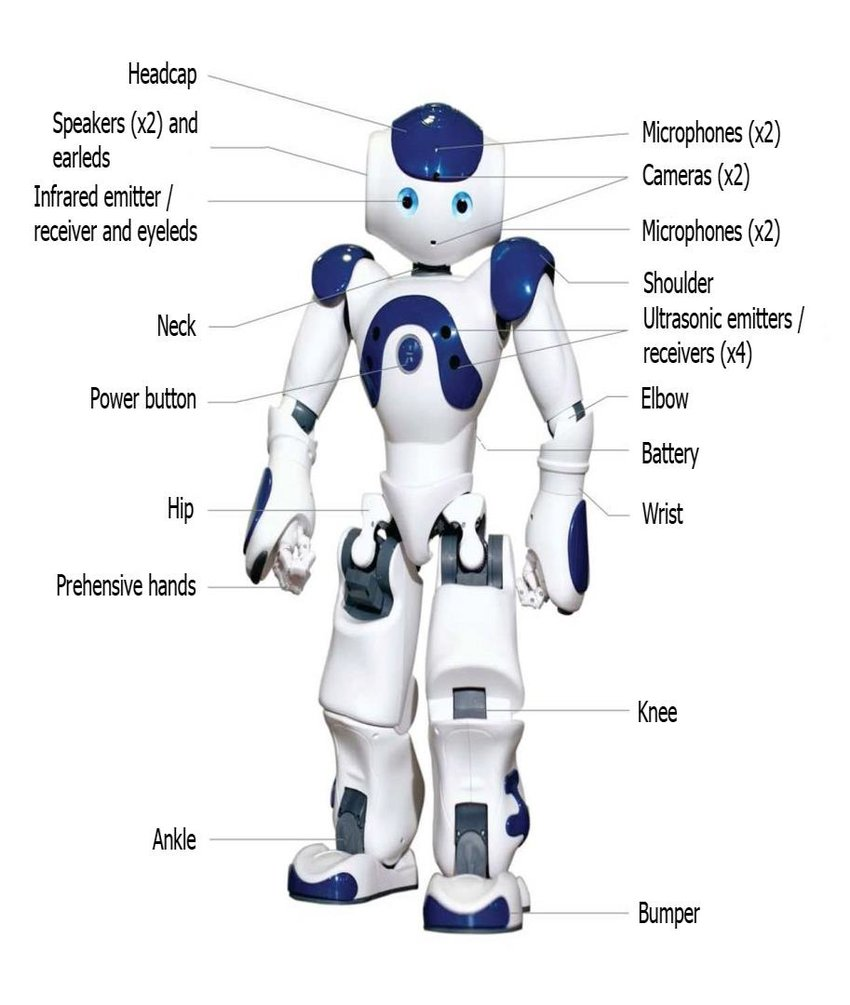
\includegraphics[width=0.6\textwidth]{nao}
    % \caption*{Fonte: Autoria própria.}
    \label{fig:nao}
\end{figure}

\subsection{Robô DARWIN-OP}
\label{ssec:darwin}

O Darwin-OP (Dynamic Anthropomorphic Robot with Intelligence-Open Platform)  é um pequeno humanoide desenvolvido pela Robotis. Ele tem 20 graus de liberdade e pesa 2.9kg, possui uma camera HD, giroscópio, acelerômetro e um microfone stereo. O Darwin é capaz de andar, falar e dançar sendo bastante utilizado por pesquisadores e programadores.

\begin{figure} [H]
    \centering
    \caption{Robô Darwin-OP}
    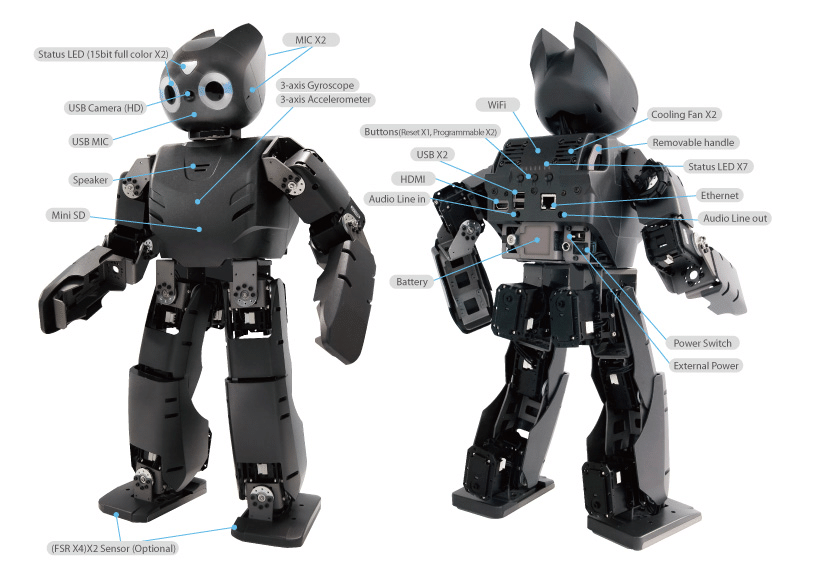
\includegraphics[width=0.8\textwidth]{darwin}
    % \caption*{Fonte: Autoria própria.}
    \label{fig:darwin}
\end{figure}

\subsection{Robô LOLA}
\label{ssec:lola}

O Lola é um robô humanoide desenvolvido na Universidade Tecnica de Munich (TUM) e financiado pela Funfação de pesquisa alem (DFG), utilizado em pesquisas sobre a dinâmica e aspectos de controle da locomoção bípede. A versão do Lola apresentada na figura X possui 24 graus de liberdade, uma altura de 180cm e pesa aproximadamente 60kg. O seu design foi projetado para possuir pouco peso, uma regidez efetiva alta, pernas com uma inércia baixa e o centro de gravidade alto. Com relação aos sensores utilizados pelo robô, o Lola possui enconders nos eixos dos seus motores e sensores de força/torque (FTS) customizados em seus pés, apresenta uma IMU em seu torso e uma câmera Intel RealSense em sua cabeça. É um robô versátil, com um design projetado para demonstrar uma caminhada bípede rápida.

\begin{figure} [H]
    \centering
    \caption{Robô LOLA}
    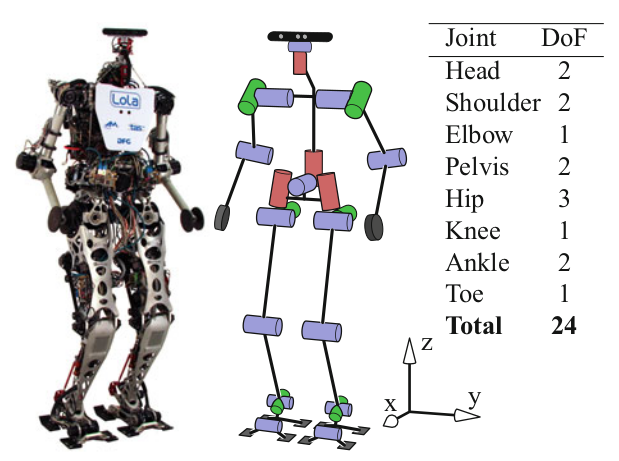
\includegraphics[width=0.8\textwidth]{lola}
    % \caption*{Fonte: Autoria própria.}
    \label{fig:lola}
\end{figure}

\subsection{Robô HUBO 2}
\label{ssec:hubo}

O HUBO 2 foi desenvolvido no laboratório HUBO no KAIST (Korean Advanced Institute os Science and Technology), na Coréia do Sul. Ele possui 125cm, pesa 45kg e possui 40 graus de liberdade. O seu design tinha como objetivo ser bem leve, o que permitiu que o HUBO 2 fosse capaz de correr em uma velocidade de 3.6 km/h. O seu sistema de percepção é composto por câmeras, sensores de inércia, inclinação e  força/torque. O seu grande diferencial em relação a outros robôs bípedes é a capacidade de utilizar uma marcha com pernas esticadas.

\begin{figure} [H]
    \centering
    \caption{Robô HUBO 2}
    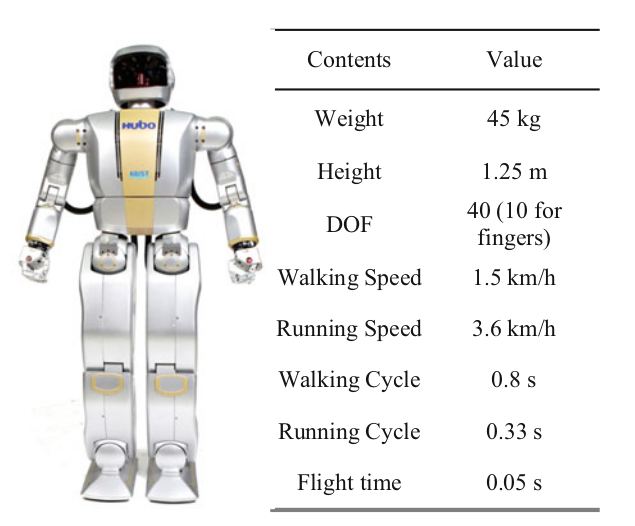
\includegraphics[width=0.8\textwidth]{hubo2}
    % \caption*{Fonte: Autoria própria.}
    \label{fig:hubo2}
\end{figure}


\section{Estudo das funcionalidades}
\label{sec:robos}

\subsection{Percepção}
\label{ssec:percepcao}

Os sensores comumente usados nos robôs humanóides podem ser classificados em dois grupos, os sensores proprioceptivos são utilizados para medir os estados de cada junta e do corpo do robô e os sensores exteroceptivos utilizados para obter informações do ambiente. São utilizados sensores internos para medir o estado do robô, como ângulos, velocidades e torques das juntas. Para detectar informações da postura do robô, utiliza-se os sensores IMU, incluindo acelerômetros e giroscópios. Enquanto, a interação entre o robô e o ambiente podem ser detectados por meio de sensores táteis e de força/torque. E, as câmeras e sensores de alcance medem e estimam as informações do ambiente ao redor do robô. 

\begin{figure} [H]
    \centering
    \caption{Classificação dos sensores}
    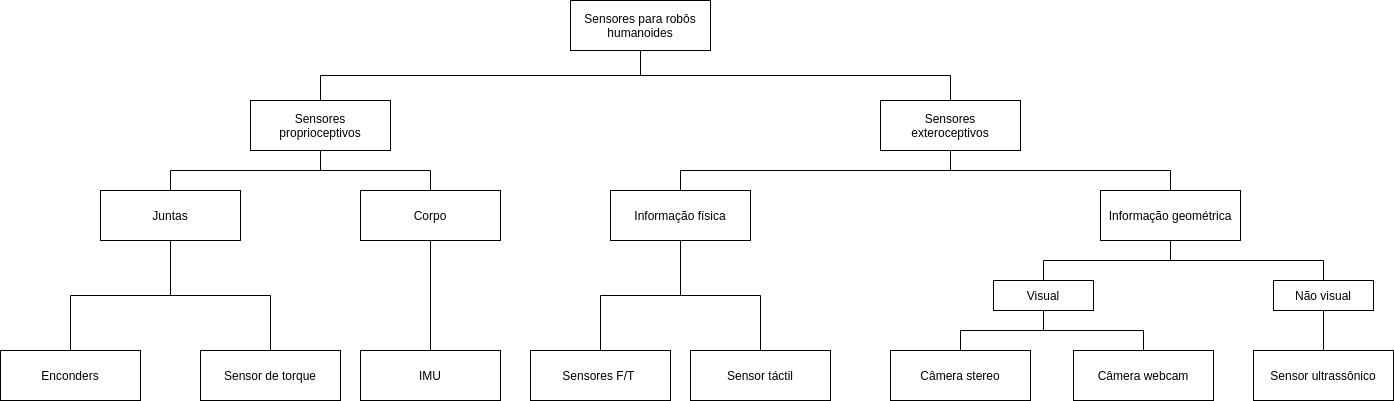
\includegraphics[width=0.8\textwidth]{sensores}
    % \caption*{Fonte: Autoria própria.}
    \label{fig:sensors}
\end{figure}

Segundo (Humanoid robot Lola: Design and walking control) o sistema de sensores do LOLA é otimizado para qualidade de sinal e largura de banda. Sensores angulares absolutos nos eixos de saída de todas as juntas compensam as elasticidades e não linearidades nos trens de força e permitem que o robô (teoricamente) comece a partir de posições arbitrárias. Dois sensores de força / torque de seis eixos feitos sob medida são fortemente integrados à estrutura do pé. Um erro de calibração de menos de 0,5 é obtido aplicando muitos casos de carga diferentes. Com um peso total de 395 g, o sensor inclui uma proteção contra sobrecarga e todos os componentes eletrônicos necessários. A unidade de medição inercial (IMU) estima a orientação e as velocidades angulares da parte superior do corpo. Visto que a precisão e a qualidade do sinal do IMU afetam consideravelmente o desempenho do controlador de estabilização, escolhemos IMU de alta precisão com giroscópios de fibra ótica e acelerômetros MEMS.

No projeto desevolvido por (Motion  planning  of  a  bipedal  walking  robot  with  leg-mounted ultrasonic  sensors  -  An  experimental  study) quatro sensores ultrassônicos, dois em cada perna, são usados para feedback da posição para caminhar e girar. O acelerômetro é usado para medir o ângulo de inclinação e para detectar a queda instantânea do robô. Sensores Resistivos de Força (FSR) são usados para determinar o centro de pressão (COP) que por sua vez é usado para calcular o ZMP do robô.


\subsection{Mecânismos}
\label{ssec:mec}

Um robô humanóide tem o formato do corpo semelhante ao de um corpo humano e tem como base a literatura sobre a análise e coordenação da marcha humana. Eles possuem um grande número de graus de liberdade (DOF), para serem capazes de realizar um movimento bípede semelhante ao humano. Para que este movimento seja mais natural e flexível, segundo (Robô humanóide Lola: Design e controle de caminhada), recomenda-se considerar uma configuração redundante com DOFs adicionais.
Para melhorar a dinâmica das pernas do robô deve-se garantir uma regidez mecânica suficiente, centro de massa alto e baixos momentos de inércia dos elos das pernas.
O objetivo básico do projeto , é, portanto, equilibrar a rigidez estrutural e o desempenho do atuador com a leveza dos componentes mecânicos.
A estrutura mecânica do Lola, por exemplo, é caracterizado pelo design leve e consistente com alta rigidez efetiva.
São utilizados servo atuadores leves e a inércia resultante das pernas é minimizada por um design sofisticado da estrutura e mecanismos de acionamento, resultando em um comportamento de aceleração superior.

\subsection{Controle}
\label{ssec:control}



%******************************************************************

\section{Mapa conceitual do estudo}
\label{sec:mapa}



%******************************************************************

\section{Organização e compartilhamento dos dados}
\label{sec:org}


%******************************************************************

\chapter{Conclusão}
\label{chap:conclu}


\section{Considerações finais}
\label{sec:consider}